%Template pembuatan proposal skripsi.
\documentclass{jtetiproposalskripsi}

%-----------------------------------------------------------------
%Disini awal masukan untuk data proposal skripsi
%-----------------------------------------------------------------
\titleind{RANCANG BANGUN SISTEM MONITORING RUANGAN DENGAN MENGGUNAKAN WEBCAM BERBASIS OPENWRT}

\fullname{DEFRI YOGA PRATAMA}

\idnum{111065 1188}

\approvaldate{20 Desember 2014}

\degree{Sarjana Teknik Informatika}

\yearsubmit{2014}

\program{Teknik Informatika}

\headprogram{Sarjiya, S.T., M.T., Ph.D.}

\dept{Teknik Informatika}

\firstsupervisor{Sigit Basuki Wibowo, S.T., M.Eng.}
\firstnip{1976 0501 2002 12 1 002}

\secondsupervisor{Bimo Sunarfri Hantono, S.T., M.Eng.}
\secondnip{1977 0131 2002 12 1 003}


%-----------------------------------------------------------------
%Disini akhir masukan untuk data proposal skripsi
%-----------------------------------------------------------------

\begin{document}

\cover

\approvalpage

%-----------------------------------------------------------------
%Disini akhir masukan untuk muka skripsi
%-----------------------------------------------------------------

%-----------------------------------------------------------------
%Disini awal masukan Intisari
%-----------------------------------------------------------------
\begin{abstractind}
Penggunaan teknologi CCTV semakin mempermudah pengguna dalam melakukan pengawasan dan pemantauan suatu ruangan. Namun kekurangan CCTV adalah harganya yang masih belum terjangkau oleh semua lapisan masyarakat. Karena hal tersebut, maka perlu dibangun sistem baru yang memiliki fitur sama dengan alat CCTV yang beredar namun dengan harga yang lebih terjangkau. 

Sistem baru ini dibangun dengan memanfaatkan sistem operasi openWRT. Sistem operasi openWRT akan dipasang pada sebuah router wireless dengan beberapa alat tambahan yang mendukung fungsionalitasnya seperti speaker, modem gsm, webcam dan flashdrive.

sistem yang dihasilkan akan memiliki kemampuan mendeteksi gerakan, sistem juga mampu mendeteksi gambar dan video ketika terdeteksi gerakan yang mencurigakan. Selain itu, sistem ini juga memiliki beberapa fitur lain seperti peringatan alarm, peringatan melalui sms, laporan ke e-mail pengguna, dan kemudahan akses melalui WIFI dan internet.


\bigskip
\textbf{Kata kunci} : CCTV, OpenWRT, Router Wireless.
\end{abstractind}
%-----------------------------------------------------------------
%Disini akhir masukan Intisari
%-----------------------------------------------------------------

\tableofcontents
\addcontentsline{toc}{chapter}{DAFTAR ISI}
\selectlanguage{bahasa}\clearpage\pagenumbering{arabic}\setcounter{page}{1}

%-----------------------------------------------------------------
%Disini awal masukan untuk Bab
%-----------------------------------------------------------------
\chapter{LATAR BELAKANG}

\section{Latar Belakang Masalah}
Seiring dengan era globalisasi dan peningkatan pertumbuhan ekonomi, mengakibatkan manusia untuk cenderung bertindak konsumtif. Bahkan sifat konsumtif ini tidak memandang apakah harta bendayang dimmiliki itu hak miliknya atau milik orang lain sehingga mengakibatkan terjadinya kasus krimminal, seperti pemcurian.

Dilain sisi, kemajuan teknologi melahirkan sistem \emph{monitoring} dengan menggunakan perangkat \emph{Closed Circuit Television} (CCTV). Penggunaan perangkat ini dapat mempermudah dalam memantau situasi dan kondisi suatu ruangan, sehingga dapat mencegah terjadinya suatu tindak kejahatan. Namun demikian,  harga CCTV yang mahal membuat perangkat ini belum bisa dijangkau semua orang.

Dengan dua latar belakang tersebut penulis merasa perlu membangun sebuah sistem yang mampu dijadikan sebagai sarana \emph{monitoring} ruangan yang mudah diakses, praktis, dan hemat. Sistem \emph{monitoring} ruangan ini menggunakan perangkat nirkabel yang akan dimodifikasi dan disesuaikan dengan kebutuhan pengguna. Diharapkan dengan teknologi nirkabel ini sistem akan menjadi lebih praktis dan mudah diakses dari mana saja.



\section{Tujuan Penelitian}
Adapun tujuan dari penelitian ini adalah Membuat system monitoring ruangan dengan openWRT yang mampu mendeteksi gerakan pada suatu ruangan. Memberikan info secara realtime tentang keadaan ruangan sehingga tindakan pencegahan dapat segera dilakukan. Dan Memberikan alternatif sistem sistem monitoring ruang yang hemat dan praktis.



\section{Manfaat Penelitian}
Manfaat dari penelitian ini adalah mempermudah pengguna dalam melakukan pengawasan terhadap suatu ruangan sehingga tindakan pencegahan terhadap hal-hal yang tidak diinginkan dapat dilakukan secepatnya

%-------------------------------------------------------------------------------
\chapter{TINJAUAN PUSTAKA DAN DASAR TEORI}                

\section{Tinjauan Pustaka}
Penelitian yang berhubungan dengan topik yang penulis angkat salah satunya penelitian yang berjudul \emph{''Aplikasi Computer Vision Untuk Mendeteksi Gerakan Pada Sistem Keamanan Rumah Menggunakan Sensor Kamera''} (Sigit, 2011). Penelitian tersebut membahas tentang perancangan aplikasi pendeteksi gerak dengan menggunakan sensor input berupa webcam dan memiliki fitur SMS, dokumentasi keadaan ruangan dan Email. Aplikasi ini dibangun dengan menggunakan tool Delphi.

Penelitian kedua berjudul \emph{''Perancangan Sistem Keamanan Rumah menggunakan Perangkat Nirkabel berbasis Openwrt''} (Romi,2011). Penelitian tersebut membahas tentang pembuatan system keamanan rumah dengan menggunakan router TP LINK WR1043ND dengan firmware Open WRT. Fitur yang ada antara lain sensor input menggunakan kabel lan dan router, webcam untuk merekam keadaan rumah, soundcard sebagai output alarm dan sms gateway untuk memberikan informasi kepada pemilik rumah. 

Penelitian ketiga yang masih memiliki kaitan yaitu penelitian yang berjudul \emph{''Prototype System Sekuriti Ruangan Berlapis Berbasis Mikrokontroller avr-atmega16 Dan Jaringan Syaraf Tirua''} (Wirawan, 2012). Penelitian ini membahas tentang perancangan system keamanan ruangan dengan memanfaatkan sensor elektronik berupa sensor inframerah dan webcam sebagai pendeteksi gerak. Sistem ini dibangun diatas mikrokontroler atmega16 dan ditunjang dengan jaringan syaraf tiruan.  

\section{Landasan Teori}
\subsection{Jaringan Wireless LAN }
Jaringan Wireless LAN (WLAN) merupakan salah satu pengembangan dari jaringan LAN. Secara harfiah, jaringan WLAN merupakan jaringan yang memungkinkan dua mesin atau lebih untuk berkomunikasi menggunakan protokol jaringan standar, dengan penggunaan media transmisi gelombang elektromagnetik berupa gelombang mikro atau gelombang radio (Wagito, 2007).

Komunikasi jaringan WLAN ini menggunakan frekuensi khusus supaya tidak terjadi interferensi dengan frekuensi alat lain. Frekuensi yang boleh digunakan disebut ISM band. ISM merupakan singkatan dari Industrial, Scientific and Medical. Frekuensi yang biasa digunakan oleh jaringan WLAN antara lain 900Mhz, 2.4 Ghz dan 5.8 Ghz. Teknologi utama yang digunakan untuk membuat jaringan WLAN adalah protokol 802.11, atau yang sering disebut dengan Wireless Fidelity (WIFI).


\subsection{Pemograman Bash Shell}
Secara harfiah, Shell merupakan program penerjemah perintah yang menjembatani user dengan sistem operasi (Yuliardi,2002). Pada umumnya, shell menyediakan prompt sebagai user interface, prompt digunakan sebagai tempat user bekerja mengetikkan perintah-perintah yang diinginkan baik berupa perintah internal shell maupun external shell. Disamping itu, shell mampu mendukung user untuk menyusun beberapa perintah pada sebuah atau beberapa file menggunakan teks editor kemudian dieksekusi layaknya sebuah program. Fitur inilah yang membuat shell disebut shell scripting. Karena dijalankan di atas linux yang menggunakan shell Bourne Again Shell (Bash) maka shell scripting disebut juga bash scripting.


\subsection{Pemograman PHP}
PHP (Hypertext Preposessor) adalah sebuah bahasa scripting yang menyatu dengan HTML (kode dasar web) dan dijalankan pada server side. Dengan begitu maka semua sintak php yang diberikan akan sepenuhnya dijalankan pada server, sedangkan hasil dari sintak tersebut akan ditampilkan pada browser (Wardana, 2010) Salah satu keunggulan PHP dibanding dengan bahasa pemrograman yang lain adalah PHP merupakan bahasa pemrograman opensource dan dapat diperoleh secara gratis. Walaupun gratis, namun PHP sangat powerfull. Dibuktikan dengan banyaknya website yang menggunakan PHP. PHP juga sudah mendukung OOP (Object Oriented Programming) sehingga maintenance kode menjadi lebih mudah.


\subsection{MySQL}
MySQL merupakan relational database management system (RDBMS) yang multithread dan open source, dibuat oleh Michael Widenius pada tahun 1995. Perusahaan yang memiliki dan mengembangkan MySQL adalah MySQL AB, yang merupakan anak perusahaan dari Sun Microsystems (Dyer,2008) MySQL tergolong sebagai database server yang andal, dapat menangani database yang besar dengan kecepatan tinggi, mendukung banyak sekali fungsi untuk mengakses database dan sekaligus mudah digunakan. MySQL menggunakan bahasa SQL (Structure Query Language) yaitu bahasa pemrogaman standar yang digunakan untuk mengakses server database. (Kadir, 2008)


\subsection{Email}
Email atau electronik mail merupakan sebuah protokol layanan pengiriman surat elektronik yang dikirim melalui internet. Untuk dapat mengirim suatu email, seorang mengguna harus mendaftarkan dirinya ke penyedia layanan untuk mendapatkan alamat email. Setelah mendaftarkan diri maka pengguna akan mendapatkan alamat email dengan format username@server.domain . Alamat inilah yang digunakan sebagai identitas dalam proses pengiriman email.

Sebuah protokol digunakan dalam proses pengiriman email ini. Protokol tersebut dinamakan SMTP (Simple Mail Transfer Protocol). Protokol ini telah menjadi sebuah aturan dasar yang disepakati untuk pengiriman email. Sehingga semua aplikasi email pasti menggunakan protokol ini.


\subsection{SMS (Short Message Service)}
SMS merupakan teknologi yang memungkinkan antar telepon genggam untuk saling mengirim dan menerima pesan. Pengiriman SMS dahulu hanya menggunakan jalur channel signal GSM (Global System for Mobile Communication), namun sekarang SMS telah mendukung pengiriman melalui teknologi GPRS dan CDMA. Pesan yang dapat dikirim dibatasi dalam satu paket/frame yang berkapasitas maksimal 140 byte atau 140 karakter huruf latin atau 70 karakter alfabet non latin seperti alfabet Arab dan Cina.


\subsection{OpenWRT}
OpenWRT adalah sebuah sistem operasi untuk \emph{embedded device} yang berbasis pada Linux kernel. OpenWRT pada umumnya digunakan dalam routing \emph{network traffic}. Komponen-komponen utamanya adalah Linux kernel, util-linux, uClibc dan BusyBox. Semua komponen sudah dioptimalkan dan dimampatkan untuk bisa muat dalam \emph{router} rumahan yang memiliki keterbatasan media penyimpan dan memori. OpenWRT dapat dikonfigurasikan melalui antarmuka \emph{command-line} (\emph{ash shell}), seperti dapat dilihat pada Gambar \ref{openwrt}, atau dengan antarmuka Web (LuCI). Terdapat kurang lebih 3.500 paket-paket perangkat lunak tambahan yang tersedia untuk diinstal melalui sistem manajemen paket \emph{opkg}.

\begin{figure}[ht!]
  \centering
    
\includegraphics[width=10cm]{gambar/openwrt}
    \caption{Tampilan antarmuka \emph{command-line} OpenWRT versi \emph{BackFire}.}
    \label{openwrt}
\end{figure}

OpenWRT dapat berjalan pada router CPE (\emph{Customer Premised Equipment}), \emph{gateway} residensial, komputer saku (seperti Ben NanoNote), dan komputer jinjing. OpenWRT juga dapat berjalan pada komputer konvensional atau komputer dengan arsitektur x86. Banyak \emph{patch} dari kode sesumber berbasis OpenWRT yang diubah kedalam Linux kernel utama.


\subsection{Motion}
Motion merupakan suatu aplikasi yang mampu memonitoring sinyal video dari sebuah kamera dan mampu mendeteksi perubahan yang terjadi pada potongan video.

Motion berkerja secara penuh dalam mode text dan tidak memiliki interface. Motion dikembangkan pertama kali oleh Jeroen Vreeken dan kemudian dilanjutkan oleh Folkert van Heusden dan Kenneth Lavrsen. Aplikasi Motion sendiri ditulis menggunakan bahasa C dan memiliki output berupa gambar jpg ataupun video mpg (Lavrsen, 2006)

Motion bekerja dengan membandingkan intesitas pixel dari gambar baru dengan gambar referensi (gambar lama). Ketika tidak ada perubahan intensitas pixel maka gambar referensi bernilai nol. Jika terjadi perubahan maka nilai dari gambar referensi akan berbeda. Untuk mencegah agar tidak terjadi salah deteksi maka dalam pengaturan motion perlu ditentukan batas perubahan pixel yang diperlukan agar bisa disebut gerakan. Dalam proses perbandingan ini warna dalam suatu gambar tidak diperlukan dan hanya diambil citra hitam putihnya saja.


\subsection{SSH}
SSH atau Secure Shell merupakan aplikasi yang digunakan untuk sarana login kedalam suatu mesin (komputer) dari jarak jauh dan mampu mengeksekusi perintah pada mesin tersebut (Wagito, 2007). Aplikasi ini menyediakan komunikasi yang terenkripsi antara dua host yang berada dalam jaringan sehingga memiliki keamanan yang lebih terjamin daripada telnet.

Protokol SSH mendukung beberapa penggunaan protokol enkripsi seperti DES, TripleDES, IDEA dan blowfish. Dengan beberapa protokol enkripsi tersebut maka aplikasi SSH lebih aman digunakan sebagai pengganti rlogin, rsh dan rcp.

SSH bekerja dengan menggunakan autentikasi kunci publik berbasis user (public key). Ketika ada permintaan dari klien untuk login pada host, maka host akan menghasilkan public key dan host key. Dengan menggunakan public key yang didapat maka klien akan membentuk suatu session dan mengenkripsi jalur data tersebut berdasar algoritma yang telah disepakati. Dengan begitu maka jalur data antara host dengan klien akan lebih aman karena telah terenkripsi.

%-------------------------------------------------------------------------------
\chapter{METODOLOGI}

\section{Alat dan Bahan}
Bahan yang digunakan dalam penelitian ini adalah:

\vspace{-0.5cm}

\begin{enumerate}[1.]
\begin{singlespace}
\itemsep0em
\item Router Wireless TP-LINK MR3420,
\item Flashdisk Sandisk 8GB,
\item Modem GSM Sierra,
\item Webcam X-Tech,
\item Generic USB Soundcard,
\item USB Hub Mumuksu,
\item VPS (Virtual Private Server),
\item Generic USB Soundcard.
\end{singlespace}
\end{enumerate}

\section{Langkah Kerja}
Pada penelitian ini dilakukan beberapa langkah kerja yang mengacu pada metode SDLC (System Development Life Cycle), dengan menggunakan model waterfall atau Model Sekuensial Linier (Pressman, 2005).


\begin{figure}[ht!]
  \centering
    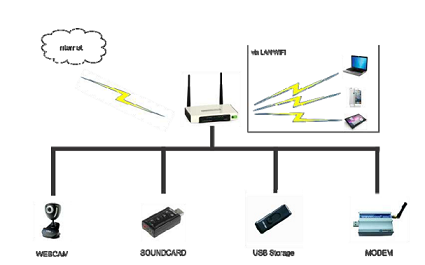
\includegraphics{gambar/konsep}
    \caption{Desain konsep Sistem Monitoring Ruangan.}
    \label{konsep}
\end{figure}


Metode Waterfall sendiri memiliki beberapa proses antara lain :

\textbf{1. Analisis}

Tahap Analisis ini dimaksudkan untuk memperoleh garis besar gambaran dari sistem monitoring ruangan yang akan dibangun. Analisis meliputi keunggulan sistem ini jika dibandingkan dengan sistem cctv yang lain, konsep dari monitoring itu sendiri dan juga untuk menganalisa tindakan dan sistem peringatan yang dilakukan oleh sistem ketika terjadi gerakan. Konsep Desain sistem ini ditunjukkan pada gambar \ref{konsep} .

\textbf{2. Perancangan}

Untuk perancangan sistem digunakan flowchart atau diagram alir untuk memperlihatkan langkah-langkah setiap proses yang terjadi pada sistem seperti pada gambar \ref{flow} . Pada tahap ini juga dilakukan perancangan untuk desain antarmuka sistem.

\begin{figure}[ht!]
  \centering
    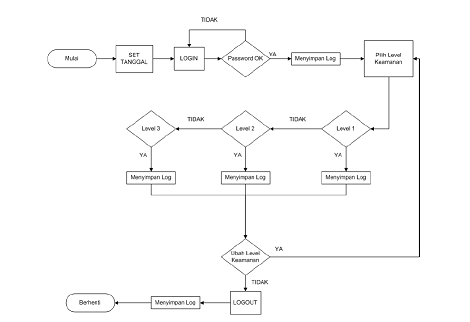
\includegraphics{gambar/flow}
    \caption{Flowchart Sistem Monitoring Ruangan.}
    \label{flow}
\end{figure}

\textbf{3. Implementasi}

Pada tahap ini, hasil perancangan sistem maupun perancangan antarmuka akan diimplementasikan dengan menggunakan PHP dan bash script.

\textbf{4. Pengujian}

Metode pengujian dilakukan untuk mengetahui apakah sistem yang dibangun sudah berjalan sesuai rencana awal atau belum. Didalam pengujian ini penulis menggunakan metode Alpha dan Beta testing dengan keterangan sebagai berikut :

\textsl{A. Alpha Testing}

Pengujian Alpha testing digunakan untuk menguji fungsionalitas dari sistem. Pengujian ini dilakukan oleh penulis dengan menggunakan 2 tingkat level keamanan yaitu level 2 dan level 3. Dipilihnya kedua level ini dikarenakan pada kedua level ini hampir semua modul dijalankan.

\textsl{B. Beta Testing}

Pengujian beta testing dilakukan secara objektif dengan menyebar kuisioner kepada responden dengan latar belakang berbeda. Pengujian ini digunakan untuk mengetahui kelebihan dan kekurangan interface pada sistem.


\section{Jadwal Kegiatan}
Penelitian direncanakan akan dilaksanakan selama enam bulan. Rincian rencana jadwal penelitian dicantumkan dalam tabel berikut.

\begin{center}
Tabel 3.1. Jadwal Penelitian.
\end{center}
\vspace{-0.5cm}
\begin{figure}[ht!]
  \centering
    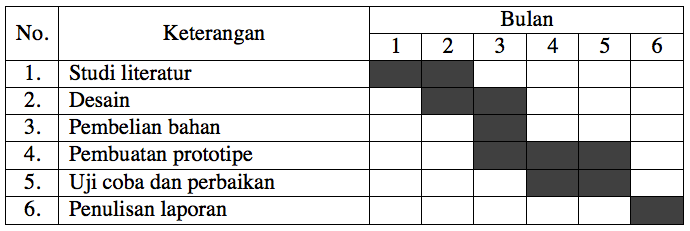
\includegraphics[width=13cm]{gambar/timeline}
\end{figure}

%-----------------------------------------------------------------
%Disini akhir masukan Bab
%-----------------------------------------------------------------

%-----------------------------------------------------------------
%Disini awal masukan untuk Daftar Pustaka
%-----------------------------------------------------------------
%%\nocite{Abel2010,Guerbas201350}
%%\bibliography{research-plan}
%%\bibliographystyle{plainnat}
\begin{thebibliography}{9}

\bibitem[satu(2014)]{satu01}
Admin, How To Send Mail with Attachment in PHP, Januari 2009 http://xahlee.info/php/, accessed December 1, 2012

\bibitem[dua(2014)]{dua02}
Cooper, Mendel. Advanced Bash-Scripting Guide. Linux Documentation Library. 2011.

\bibitem[tiga(2014)]{tiga03}
Dyer, Russel. MySQL in a Nutshell. USA: O’Reilly Media. 2008.

\bibitem[empat(2014)]{empat04}
Kadir, Abdul. Tuntunan Praktis: Belajar Database Menggunakan MySQL. Yogyakarta: Penerbit Andi. 2008.

\bibitem[lima(2014)]{lima05}
Lavrsen, Kenneth. Legacy Motion Guide for Motion versions 3.1.18 - 3.1.20. Februari 2006. http://www.lavrsen.dk foswiki/bin/view/Motion/Motion Guide 3x1x20 (accessed December 10, 2012).

\bibitem[enam(2014)]{enam06}
K. V. Kale I. K. Advances In Computer Vision And Information Technology. International Pvt Ltd. 2008.

\bibitem[tujuh(2014)]{tujuh07}
Madara, Anwar. Pengertian MySQL. Februari 2012. http://anwarmadara.blogspot.com/2012/02/pengertian-mysql.html (accessed December 10, 2012)

\bibitem[delapan(2014)]{delapan08}
Nixcraft. How To : Add Jobs To cron Under Linux or UNIX?. April 2006. http://www.cyberciti.biz/faq/how-do-i-add jobs-to-cron-under-linux-orunix-oses/ (accessed November 16, 2012)

\bibitem[sembilan(2014)]{sembilan09}
Romi, Agustian. Perancangan Sistem Keamanan Rumah menggunakan Perangkat Nirkabel berbasis Openwrt. Surabaya : Universitas Wijaya Kusuma. 2011

\bibitem[sepuluh(2014)]{sepuluh10}
Wiki. About OpenWRT. http://wiki.openwrt.org/about/start (acessed December 1,2012)

\end{thebibliography}
\addcontentsline{toc}{chapter}{DAFTAR PUSTAKA}
%-----------------------------------------------------------------
%Disini akhir masukan Daftar Pustaka
%-----------------------------------------------------------------

\end{document}